\documentclass[11pt]{article}
\usepackage[utf8]{inputenc}
\usepackage{amsmath, amssymb, bm, booktabs, graphicx, float, geometry, hyperref, enumitem, xcolor}
\geometry{margin=1.1in}
\hypersetup{colorlinks=true, linkcolor=blue!50!black, urlcolor=blue!50!black}
\setlist{itemsep=2pt, topsep=3pt}
\newcommand{\claim}[1]{\textbf{#1}}

\title{\Large Taking the Framework Apart:\\ What Each Piece Does, and What Generalizes}
\author{Working note (for me, before the next audience)}
\date{\today}

\begin{document}
\maketitle

\noindent\textbf{Purpose.} This note dismantles the model into its working parts, switches each one off in turn,
and records what happens to (i) the level of welfare losses, (ii) the optimal exchange-rate response, and (iii)
the regime ranking. It answers the questions raised after the July 22 presentation (Christian: ``how does the
optimal regime change with and without the network?''; Adam: ``what is the optimal weight on the exchange rate, and
how does it change with the network?'') and ends with a crib sheet of audience questions. All numbers come from
the 3-sector Chile calibration (the only one for which a joint rule optimization is cheap); losses are in units of
$10^{-4}$. Code: \texttt{code/opt\_rule\_point.m} (+ \texttt{\_hipi}, \texttt{\_slice}, \texttt{\_peg} variants),
\texttt{code/analysis\_opt\_rule.py}, \texttt{code/network\_anatomy.py}; raw output in \texttt{results/opt\_rule\_*.csv}.

\section{The one-paragraph version}

Four things happen in the model, and each can be isolated. (1) A \emph{production network} propagates cost shocks
between sectors. (2) \emph{Heterogeneous price stickiness} turns those cost shocks into markup dispersion in the
sticky sectors, which is what welfare penalizes. (3) The \emph{exchange rate} is a second cost-push channel,
entering every sector's Phillips curve through $\Gamma\Delta e_t$, with $\Gamma\propto\tilde A\,\bm\Omega^F$: direct
imports \emph{plus} imports inherited from suppliers. (4) A \emph{financial shock} (risk premium in UIP) moves $\Delta e_t$
or the interest rate for reasons unrelated to the real economy, and the policy rule decides which of the two moves.
The regime comparison is mostly a statement about (4) and about how aggressively the rule fights inflation; the
network and stickiness (1)--(3) decide how much an explicit exchange-rate response adds on top.

\section{The pieces, and what each contributes}

\begin{table}[H]
\centering\small
\begin{tabular}{p{3.0cm}p{4.3cm}p{6.6cm}}
\toprule
Piece & Where it lives & What it does to the results \\
\midrule
Domestic IO network $\Omega^H$ (density $\rho$) & $\mathcal V$, $\mathcal B$, $\Gamma$, Domar weights $\lambda_D$ & Raises the optimized loss ($3.7\to6.3\to9.5$ for $\rho=0,1,1.5$ at baseline shocks); raises the value of an FX response to \emph{real} shocks from 0.4\% to 12\% \\[2pt]
Heterogeneous stickiness $\hat\delta_i$ & welfare weights $\kappa_i$, DC index $\bm\phi^{DC}$ & Without it the FX term is worth less ($5.9\%\to4.2\%$ of loss at $\rho=1$; $3.3\%\to1.6\%$ at $\rho=0$) \\[2pt]
Imported inputs $\bm\Omega^F$ & $\Gamma$ & Without direct imported inputs the FX term is worth $3.6\%$ instead of $5.9\%$ (consumption-side and export channels remain) \\[2pt]
Risk-premium shock $\varepsilon^{RP}$ & UIP & Makes Peg catastrophic; gives the FX term a network-\emph{independent} value ($\approx$11\% when doubled, at every $\rho$) \\[2pt]
Debt elasticity $\Psi$ & UIP closing device & Second-order for the rule ($5.7\%$ vs $5.2\%$ for $\Psi=0.005$ vs $0.1$) \\[2pt]
Policy aggressiveness $\phi_\pi$ & rule & \emph{The} dominant lever: raising $\phi_\pi$ from $1.5$ to $\approx$20 cuts Managed's loss by 38\% and Float's by 74\% \\
\bottomrule
\end{tabular}
\caption{Anatomy of the model: effect of each ingredient (3-sector Chile, $\phi_\pi=20,\ \phi_y=1$ slice unless noted).}
\end{table}

\section{Optimal exchange-rate response with and without the network}

\subsection{Setup}

I solve the model once per structural scenario and then re-solve it on a grid of the rule
$\log(I/I^*)=\phi_\pi\pi^{DC}_t+\phi_y\tilde y_t+\phi_s\log S_t$ (451 points per scenario: $\phi_\pi\in[1.2,300]$,
$\phi_y\in[0,2]$, $\phi_s\in[0,3]$), computing welfare from analytic second moments with the model's own Domar weights
(which change with $\rho$). The baseline cell reproduces the headline managed-float loss ($10.17$). Scenarios: network
density $\rho\in\{0,0.5,1,1.5\}$ crossed with risk-premium shock size $\{0,0.5,1,2\}\times$ baseline, plus ablations.

\subsection{Result 1: the optimal rule is close to strict targeting of the divine-coincidence index}

In every scenario the loss is minimized at a very hard response to the DC-index inflation ($\phi_\pi\approx20$--$50$)
and $\phi_y\approx1$; the loss surface is flat beyond $\phi_\pi\approx20$. This is the Rubbo logic surviving in the open
economy: targeting $\pi^{DC}$ removes the productivity cost-push, and what is left is the exchange-rate channel
$\bm\phi^{DC\top}\Gamma\Delta e_t$ (the divine-coincidence breakdown result of the paper). The exchange-rate term in the rule is a
\emph{correction for that leftover}, not the main event.

\subsection{Result 2: how much the FX term is worth depends on the network, and on which shock}

\begin{figure}[H]
\centering
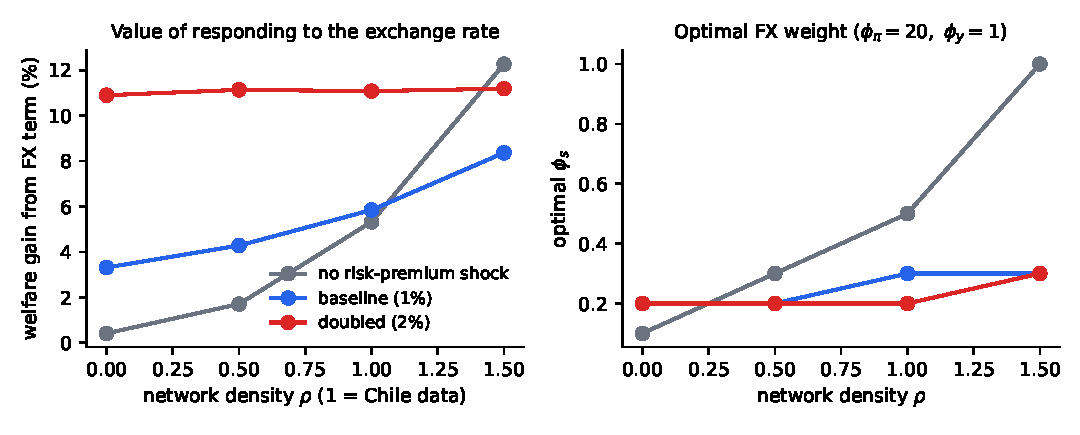
\includegraphics[width=\textwidth]{figs/opt_rule_network.pdf}
\caption{Value of adding $\phi_s>0$ to the near-optimal Taylor rule, and the optimal $\phi_s$, by network density and
risk-premium shock size ($\phi_\pi=20,\ \phi_y=1$).}
\end{figure}

\begin{table}[H]
\centering\small
\begin{tabular}{lcccc|cccc}
\toprule
 & \multicolumn{4}{c|}{Value of FX term (\% of loss)} & \multicolumn{4}{c}{Optimal $\phi_s$} \\
$\rho$ & 0 & 0.5 & 1 & 1.5 & 0 & 0.5 & 1 & 1.5 \\
\midrule
No risk-premium shock & 0.4 & 1.7 & 5.3 & 12.3 & 0.1 & 0.3 & 0.5 & 1.0 \\
Baseline (1\%) & 3.3 & 4.3 & 5.9 & 8.4 & 0.2 & 0.2 & 0.3 & 0.3 \\
Doubled (2\%) & 10.9 & 11.1 & 11.1 & 11.2 & 0.2 & 0.2 & 0.2 & 0.3 \\
\midrule
Optimized loss, baseline shocks & 3.68 & 4.58 & 6.26 & 9.50 & & & & \\
\bottomrule
\end{tabular}
\caption{Network $\times$ risk-premium grid at the near-optimal Taylor rule ($\phi_\pi=20,\phi_y=1$). ``Value'' is
the loss reduction from choosing $\phi_s^*$ rather than $\phi_s=0$. Plateau: the loss is within 1\% of its minimum over
a range of $\phi_s$ (e.g.\ $0.2$--$0.3$ at $\rho=1$), so $\phi_s^*$ is poorly identified when the gain is small.}
\end{table}

Two separable stories:
\begin{enumerate}
\item \claim{Against real shocks, the network is what makes an FX response worthwhile.} With the risk-premium shock off,
the FX term is nearly worthless without a network (0.4\%) and worth 12\% at $\rho=1.5$; the optimal weight rises
$0.1\to1.0$. Mechanism: the network lets import-cost shocks reach sticky, import-light sectors (Services) through suppliers, so
$\bm\phi^{DC\top}\Gamma$ grows with $\rho$ (the DC-residual ratio $\bm\phi^{DC\top}\Gamma/\bm\phi^{DC\top}\mathcal B$ rises from
0.15 to 0.21 over $\rho=0\to1.5$, \texttt{results/network\_anatomy.csv}) and also because every cost shock is more costly when it propagates.
\item \claim{Against the financial shock, the network is irrelevant.} The risk-premium shock moves the exchange rate directly; the
value of leaning against it is $\approx$11\% at every $\rho$ when the shock is doubled, with $\phi_s^*\approx0.2$. A policy-maker
facing mainly UIP shocks should lean against the exchange rate whether or not the economy has a production network.
\end{enumerate}
So the honest answer to ``does the optimal FX response depend on the network?'' is: \emph{yes, for real shocks; no, for financial
shocks; and in the baseline calibration (equal 1\% shocks) the gain from the FX term is modest, $3$--$8$\% of loss.}

\subsection{Result 3: the regime ranking is largely a statement about rule aggressiveness}

\begin{figure}[H]
\centering
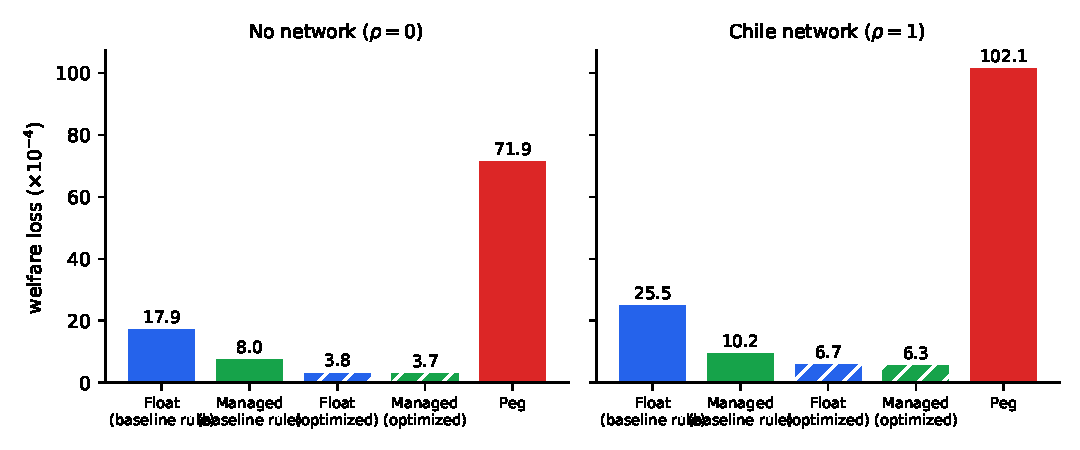
\includegraphics[width=\textwidth]{figs/opt_rule_regimes.pdf}
\caption{Welfare loss by regime with the paper's baseline rule ($\phi_\pi=1.5,\phi_y=0.5$) versus optimized rules, baseline shocks.}
\end{figure}

\begin{table}[H]
\centering\small
\begin{tabular}{lccccc}
\toprule
 & Float (base) & Managed (base) & Float (opt.) & Managed (opt.) & Peg \\
\midrule
$\rho=0$ (no network) & 17.9 & 8.0 & 3.80 & 3.68 & 71.9 \\
$\rho=1$ (Chile) & 25.5 & 10.2 & 6.65 & 6.26 & 102.1 \\
\bottomrule
\end{tabular}
\caption{Regime comparison at baseline vs.\ optimized rules (baseline shocks).}
\end{table}

The headline ``Managed beats Float by $2.5\times$'' compares a weak float rule ($\phi_\pi=1.5$) with a managed rule whose
FX term partly \emph{substitutes for} the missing inflation response. Once both are optimized, Managed beats Float by only
$3$--$6$\%. What does survive: (a) Peg is the clear loser, $16$--$20\times$ worse than an optimized rule, with or without the network,
and even with the risk-premium shock off (Peg 25.2 vs.\ 6.1 at $\rho=1$), because giving up the policy rate costs a lot against
\emph{real} shocks too; (b) the loss of every regime rises with network density, Peg fastest. \claim{The paper's regime comparison
should be presented as ``Peg vs.\ an optimized rule, with a small additional gain from an FX term'', not as ``Managed beats Float
by a wide margin''.}

\subsection{Result 4: where the import exposure sits relative to stickiness}

Christian's example (rigid ``real economy'' sector buying from a flexible import-export sector) says the \emph{location} of
exposure relative to stickiness matters. Permuting the three import shares $\{0.0767,0.1945,0.0704\}$ across sectors:
\begin{table}[H]
\centering\small
\begin{tabular}{lccc}
\toprule
Import-heavy sector & Resource (flexible) & Manufacturing (data) & Services (sticky) \\
\midrule
Loss, $\rho=1$, real shocks only & 5.75 & 6.09 & 6.79 \\
Value of FX term (\%) & 4.9 & 5.3 & 7.5 \\
\bottomrule
\end{tabular}
\end{table}
Putting the import-heavy role on the stickiest sector raises the loss by about 12\% and raises the value of an FX response by about
two points; at $\rho=0$ the same permutation moves the loss by at most $0.6$ (the effect needs the network to transmit exposure). Effects
are real but modest in this calibration, because the calibrated import shares differ by at most a factor of three and the stickiest sector
(Services) is also the one with the lowest direct import share.

\section{What generalizes, and under what conditions}

\begin{table}[H]
\centering\small
\begin{tabular}{p{4.2cm}p{4.2cm}p{4.6cm}}
\toprule
Claim & Holds when & Fails or is weak when \\
\midrule
\claim{DC breaks under an exchange-rate channel} (theory) & $\bm\Omega^F\not\propto\bm\alpha$ and some pass-through ($\Gamma\neq0$) & Pass-through is zero (full dominant-currency pricing of imports) or $\bm\Omega^F\propto\bm\alpha$ \\[3pt]
\claim{Network raises the value of an FX response to real shocks} & Stickiness is heterogeneous and import exposure is inherited through suppliers & Stickiness is uniform: gain falls to $1.6$--$4.2$\% \\[3pt]
\claim{Peg is by far the worst regime} & Any plausible rule can be chosen for the alternative; shocks can move the policy rate & Not tested: pegs with capital controls, or economies where $I^*$ shocks dominate \\[3pt]
\claim{Risk-premium shocks dominate Peg's loss} & $\sigma_{RP}$ is comparable to other shocks & $\sigma_{RP}\to0$: Peg is still $4\times$ an optimized rule but roughly equals a weak float \\[3pt]
\claim{Managed $>$ Float by a wide margin} & The float rule is unaggressive ($\phi_\pi\approx1.5$) & Both rules optimized: $3$--$6$\% only \\
\bottomrule
\end{tabular}
\end{table}

\section{Crib sheet: questions an audience will ask}

\begin{description}[leftmargin=1.2em, style=nextline]
\item[``Why does your managed float win?''] Only against a weak plain float. With the inflation response optimized
($\phi_\pi\approx20$) the gap closes to $3$--$6$\%. The robust claim is that an explicit exchange-rate term never hurts and helps most when
the network is dense or UIP shocks are large.
\item[``What is the optimal weight on the exchange rate?''] Small: $\phi_s^*\approx0.2$--$0.3$ at baseline, rising to $\approx1$ against real shocks
in dense networks. Because the loss is flat in $\phi_s$ near the optimum (within 1\% over $0.2$--$0.3$) the weight is weakly identified; the \emph{value} of the term
is the better-identified object.
\item[``Why does the network matter for the FX weight?''] Because the DC index cannot remove the exchange-rate cost-push, and its size
is $\bm\phi^{DC\top}\Gamma$, with $\Gamma\propto\tilde A\bm\Omega^F$ including inherited imports. A denser network raises the
inherited part ($\approx$27\% of Services' import exposure at $\rho=0$ vs.\ 41\% at $\rho=1$).
\item[``Is a peg ever good here?''] Not in this model: it forfeits the policy rate, and the risk-premium shock then goes straight to
the output gap. Without the shock, the peg is still $4\times$ worse than an optimized rule. Caveats: no capital controls, no credibility
benefit, no fiscal side.
\item[``Is the model over-identified (Phillips curve + UIP + law of one price)?''] No: Phillips curves price sectors, UIP prices the
currency, LOP prices imports. Together they determine inflation, the exchange rate and the rate, given the rule.
\item[``What if import prices are invoiced in dollars?''] Not modeled (producer-currency pricing). Dominant-currency pricing would weaken
$\Gamma$ for the domestic-currency exchange rate and shift weight to the dollar rate; a natural extension.
\item[``How big is each ingredient?''] See the anatomy table: $\phi_\pi$ dominates the level; the risk-premium shock dominates the Peg
loss; the network and stickiness heterogeneity decide the value of the FX term.
\item[``Does 12/33/81 sectors change this?''] The ranking is stable; Peg's loss is invariant to resolution while Float's falls
(diversification of sectoral shocks). The optimal-rule exercise has been run at 3 sectors only.
\item[``Which parameter would you estimate first?''] The risk-premium shock's volatility: it sets Peg's loss and the network-independent
part of the FX value. Then sectoral shock volatilities, which set the level of Float and Managed losses.
\end{description}

\section{Open issues in the framework itself}

\begin{itemize}
\item The optimal-rule exercise uses one 3-sector calibration and equal shock volatilities; the multi-country, many-sector version is the obvious
next run (use the same approach with simulated moments).
\item Welfare is the second-order approximation of the closed-economy form extended by the cross-sector term; the cross-sector term is
not included in the optimization grid (it adds $3$--$8$\% and does not alter rankings in the baseline).
\item Rule class is restricted to Taylor-type rules in $(\pi^{DC},\tilde y,\log S)$; a fully optimal (Ramsey) policy is not computed. The finding that
$\phi_\pi\to$ large is optimal suggests Ramsey would deliver strict DC-index targeting plus a correction for $\Gamma\Delta e_t$.
\item The optimized rule requires the central bank to observe $\pi^{DC}$, the Domar-and-stickiness-weighted index; a CPI-based rule is worse
in the earlier robustness exercise.
\end{itemize}

\end{document}
